\section{NF Module API}

\begin{figure}[!h]
\begin{subfigure}[t]{0.49\linewidth}
   \centering
   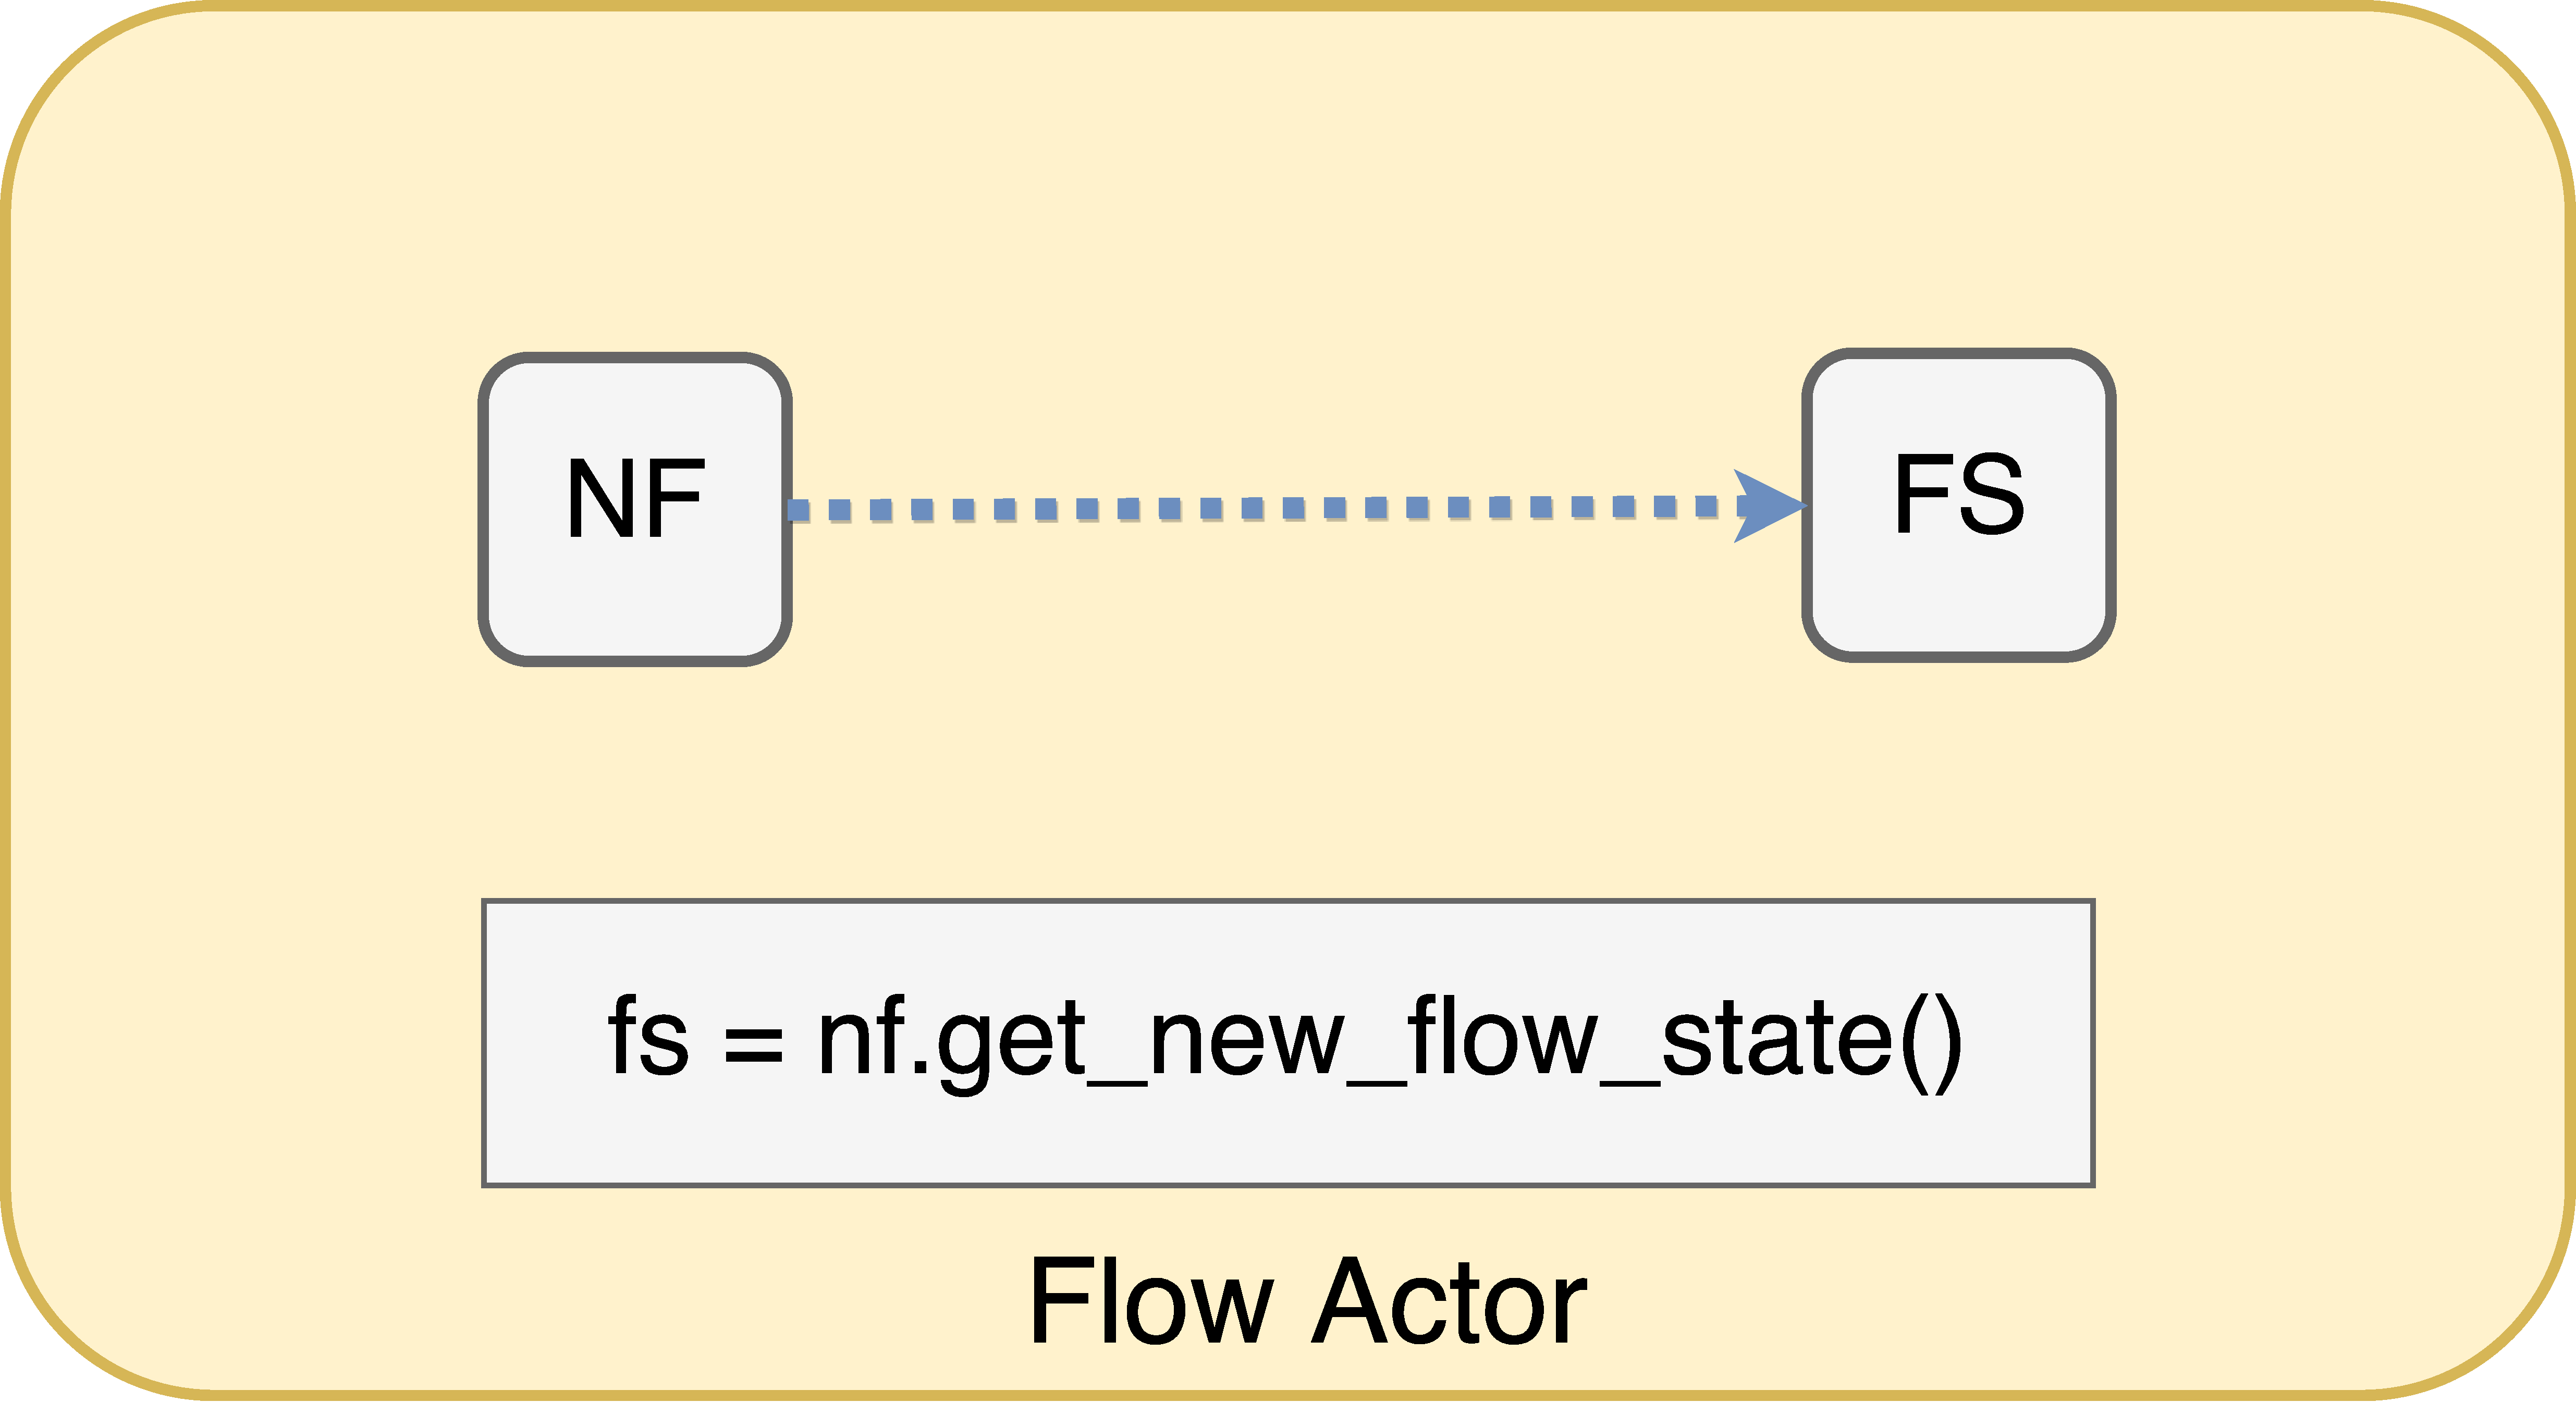
\includegraphics[width=\columnwidth]{figure/nf-module-api-init.pdf}
   \caption{The API that is used to initialize flow state when the flow actor is created.}\label{fig:init-api}
  \end{subfigure}\hfill
  \begin{subfigure}[t]{0.49\linewidth}
 \centering
   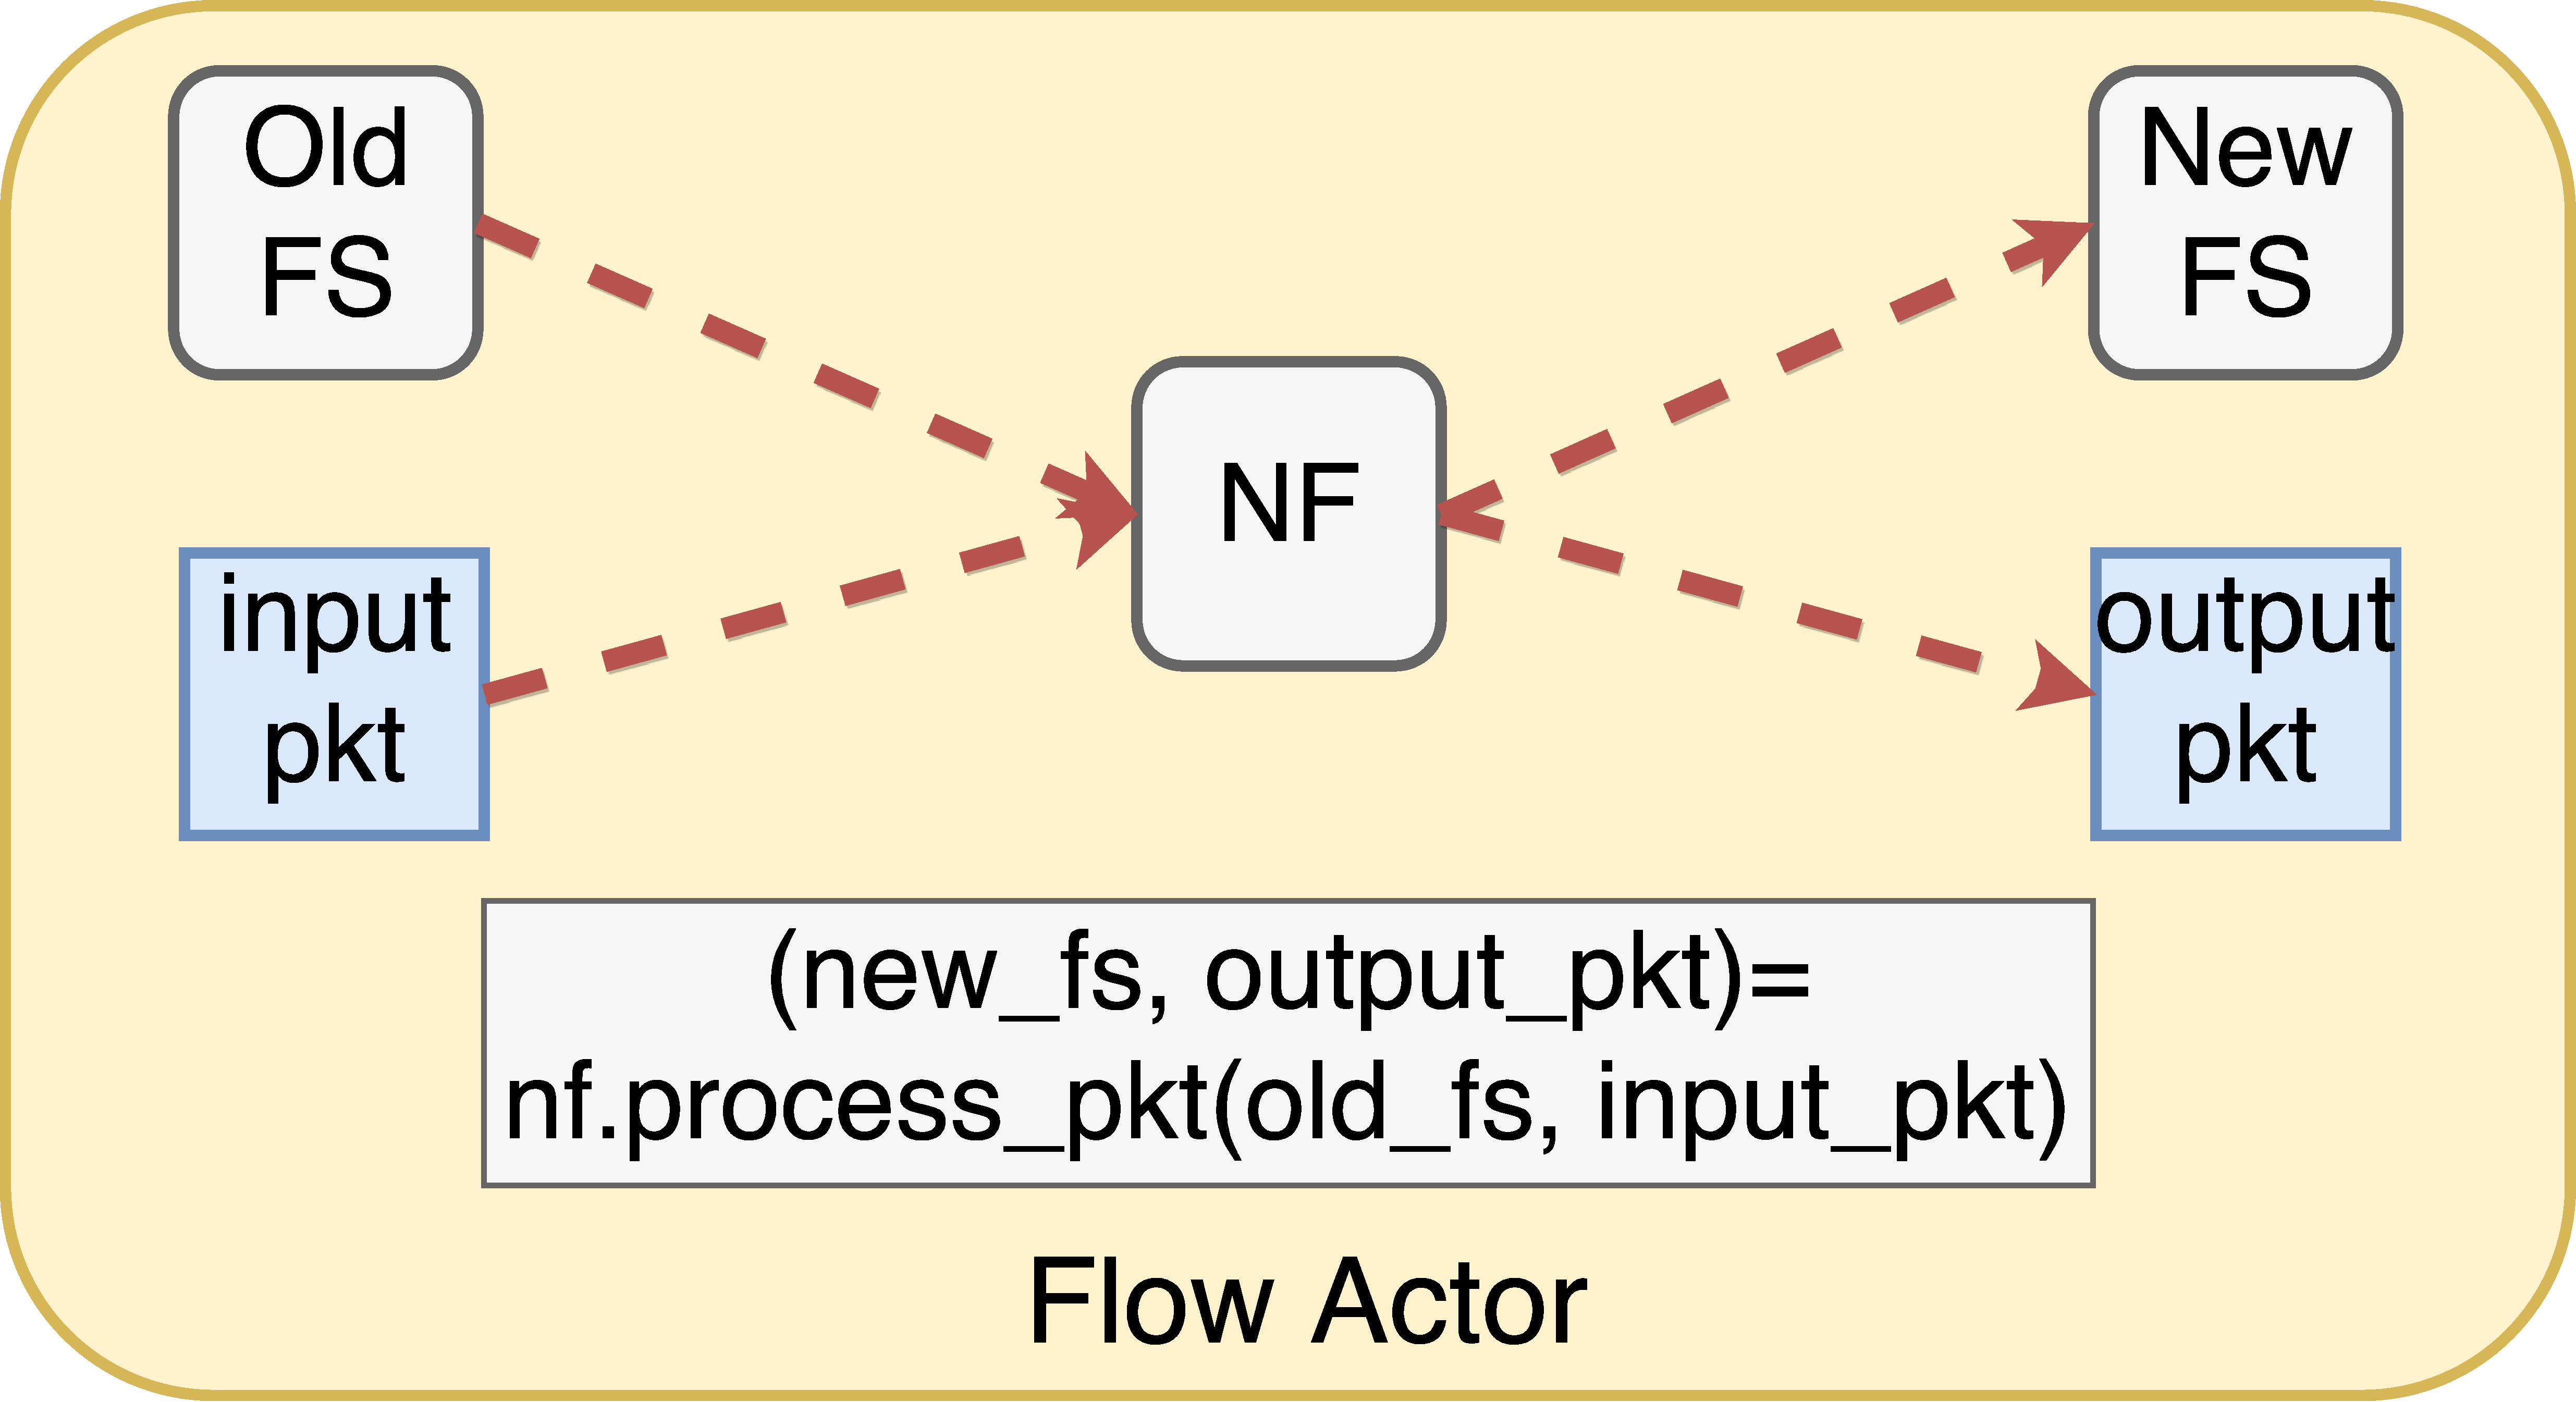
\includegraphics[width=\columnwidth]{figure/nf-module-api-process_pkt.pdf}
   \caption{The API that is used to process input packet.}\label{fig:pkt-process-api} \end{subfigure}\hfill
 \caption{The API exposed by NFActor for implementing new NF modules. (NF: Network function. FS: Flow state. pkt: packet.)}
\label{fig:api}
\end{figure}

Each NF used by NFActor is implemented as a loadable module. The runtime system could select which NF module to load and use. In order to achieve the service chain processing as indicated in figure \ref{fig:runtime-arch}, we pass in an argument indicating the composition of the service chain before initializing a runtime. The runtime guarantees that each flow actor processes the packet through each NF as indicated in the service chain. The modular NF design is similar to that in NetBricks \cite{199352}, however, NFActor modifies the interface exposed by the NF module to achieve efficient flow management.

When executing flow management tasks, flow actor must be able to extract and transmit the flow states of all the NFs on the service chain, without disturbing the normal service chain processing. To speed up this process, we propose to separate the flow state with the processing logic of the NF module, and store the flow state inside the flow actor.

We summarize the core APIs used by NFActor to construct new NF modules in figure \ref{fig:api}. Using these APIs, the flow actor could acquire a new flow state when it is created. When the flow actor processes a packet, the flow actor passes the current flow state and the input packet together into the processing logic of a NF module. The processing logic could directly update the flow state according to the input packet. Since the flow state is stored by the flow actor, the flow actor could directly manipulate its flow state when executing flow management tasks, without disturbing the NF processing logic.

Even though this design facilitates flow management tasks, it has its own limitation. Using this design, it is hard to extract and tranismit shared states. However, it is a complicated tasks to guaratee the consistency of shared states when managing a single flow. It may require multiple synchronizations, thereby affecting the processing speed of a single flow management task. Sice our primary goal when designing NFActor is to provide a high performance exeuction context, we do not aim to synchronize shared state. Instead, when flow management affects the consistency of the shared state, we could explicitly notify the NF about the result of flow management tasks and let NF module to handle the inconsistecy.
